\documentclass[portrait,final,a0paper,fontscale=0.3]{baposter}
% Currently set to 24" wide by 36" tall (archD).
% See baposter.cls for info on changing paper dimensions

\usepackage{calc}
\usepackage{graphicx}
\usepackage{amsmath}
\usepackage{amssymb}
\usepackage{relsize}
\usepackage{multirow}
\usepackage{rotating}
\usepackage{bm}
\usepackage{url}

\usepackage{graphicx}
\usepackage{multicol}
\usepackage{amsthm}
\usepackage{amssymb}
\usepackage{mathtools}
\DeclarePairedDelimiter\abs{\lvert}{\rvert}
\DeclarePairedDelimiter\norm{\lVert}{\rVert}
\DeclarePairedDelimiter\inner{\langle}{\rangle}
\def\P{\mathcal{P}}
\DeclareMathOperator*{\argmin}{argmin}
\theoremstyle{definition}
\newtheorem{definition}{Definition}
\newtheorem{proposition}{Proposition}
\newtheorem{example}{Example}
\newtheorem{lemma}{Lemma}
\newtheorem{corollary}{Corollary}
\newtheorem{theorem}{Theorem}
\usepackage{algorithm}
\usepackage{algorithmic}
\makeatletter
\newcommand{\algorithmicfunction}{\textbf{function}}
\newcommand{\algorithmicendfunction}{\algorithmicend\ \algorithmicfunction}
\newenvironment{ALC@func}{\begin{ALC@g}}{\end{ALC@g}}
\newcommand{\FUNCTION}[2][default]{\ALC@it\algorithmicfunction\ #2\ %
\textbf{:}%
\ALC@com{#1}\begin{ALC@func}}
\ifthenelse{\boolean{ALC@noend}}{
    \newcommand{\ENDFUNCTION}{\end{ALC@func}}
  }{
    \newcommand{\ENDFUNCTION}{\end{ALC@func}\ALC@it\algorithmicendfunction}
  }
\makeatother

%\usepackage{times}
%\usepackage{helvet}
%\usepackage{bookman}
\usepackage{palatino}

\newcommand{\captionfont}{\footnotesize}

%%%%%%%%%%%%%%%%%%%%%%%%%%%%%%%%%%%%%%%%%%%%%%%%%%%%%%%%%%%%%%%%%%%%%%%%%%%%%%%%
%%%% Some math symbols used in the text
%%%%%%%%%%%%%%%%%%%%%%%%%%%%%%%%%%%%%%%%%%%%%%%%%%%%%%%%%%%%%%%%%%%%%%%%%%%%%%%%

%%%%%%%%%%%%%%%%%%%%%%%%%%%%%%%%%%%%%%%%%%%%%%%%%%%%%%%%%%%%%%%%%%%%%%%%%%%%%%%%
% Multicol Settings
%%%%%%%%%%%%%%%%%%%%%%%%%%%%%%%%%%%%%%%%%%%%%%%%%%%%%%%%%%%%%%%%%%%%%%%%%%%%%%%%
\setlength{\columnsep}{1.5em}
\setlength{\columnseprule}{0mm}

%%%%%%%%%%%%%%%%%%%%%%%%%%%%%%%%%%%%%%%%%%%%%%%%%%%%%%%%%%%%%%%%%%%%%%%%%%%%%%%%
% Save space in lists. Use this after the opening of the list
%%%%%%%%%%%%%%%%%%%%%%%%%%%%%%%%%%%%%%%%%%%%%%%%%%%%%%%%%%%%%%%%%%%%%%%%%%%%%%%%
\newcommand{\compresslist}{%
\setlength{\itemsep}{1pt}%
\setlength{\parskip}{0pt}%
\setlength{\parsep}{0pt}%
}

%%%%%%%%%%%%%%%%%%%%%%%%%%%%%%%%%%%%%%%%%%%%%%%%%%%%%%%%%%%%%%%%%%%%%%%%%%%%%%
%%% Begin of Document
%%%%%%%%%%%%%%%%%%%%%%%%%%%%%%%%%%%%%%%%%%%%%%%%%%%%%%%%%%%%%%%%%%%%%%%%%%%%%%

\begin{document}

%%%%%%%%%%%%%%%%%%%%%%%%%%%%%%%%%%%%%%%%%%%%%%%%%%%%%%%%%%%%%%%%%%%%%%%%%%%%%%
%%% Here starts the poster
%%%---------------------------------------------------------------------------
%%% Format it to your taste with the options
%%%%%%%%%%%%%%%%%%%%%%%%%%%%%%%%%%%%%%%%%%%%%%%%%%%%%%%%%%%%%%%%%%%%%%%%%%%%%%
% Define some colors

\definecolor{stevensred}{HTML}{82318E}
\definecolor{stevensgray}{rgb}{0.60392, 0.596, 0.60392}

%%
\begin{poster}%
  % Poster Options
  {
  % Show grid to help with alignment
  grid=false,
  % Column spacing
  colspacing=1em,
  % Color style
  bgColorOne=white,
  bgColorTwo=white,
  borderColor=stevensgray,
  headerColorOne=stevensred,
  headerColorTwo=stevensred,
  headerFontColor=white,
  boxColorOne=white,
  boxColorTwo=stevensgray,
  % Format of textbox
  textborder=rectangle,
  % Format of text header
  eyecatcher=true,
  headerborder=closed,
  headerheight=0.1\textheight,
%  textfont=\sc, An example of changing the text font
  headershape=rectangle,
  headershade=shadelr,
  headerfont=\Large\bf\textsc, %Sans Serif
  textfont={\setlength{\parindent}{1.5em}},
  boxshade=plain,
%  background=shade-tb,
  background=plain,
  linewidth=2pt
  }
  % Eye Catcher
  {
  		
\includegraphics[height=9.0em]{thu.jpg}
  %\begin{minipage}{8em}	
  %   \hfill\vspace{1in}
  %\end{minipage} 
  } % Empty space, replace with image if desired
  % Title
  {\bf \textsc{ Info-Detection: An Information-Theoretic Approach to Detect Outlier } }
  % Authors
  {\textsc{  Feng Zhao, Fei Ma, Yang Li, Shao-Lun Huang and Lin Zhang \\ Tsinghua-Berkeley Shenzhen Institute, Tsinghua University}}
  % University logo
  {% The makebox allows the title to flow into the logo, this is a hack because of the L shaped logo.
%    \includegraphics[height=9.0em]{../logo_forum.png}
  }

%%%%%%%%%%%%%%%%%%%%%%%%%%%%%%%%%%%%%%%%%%%%%%%%%%%%%%%%%%%%%%%%%%%%%%%%%%%%%%
%%% Now define the boxes that make up the poster
%%%---------------------------------------------------------------------------
%%% Each box has a name and can be placed absolutely or relatively.
%%% The only inconvenience is that you can only specify a relative position 
%%% towards an already declared box. So if you have a box attached to the 
%%% bottom, one to the top and a third one which should be in between, you 
%%% have to specify the top and bottom boxes before you specify the middle 
%%% box.
%%%%%%%%%%%%%%%%%%%%%%%%%%%%%%%%%%%%%%%%%%%%%%%%%%%%%%%%%%%%%%%%%%%%%%%%%%%%%%
    %
    % A coloured circle useful as a bullet with an adjustably strong filling
    \newcommand{\colouredcircle}{%
      \tikz{\useasboundingbox (-0.2em,-0.32em) rectangle(0.2em,0.32em); \draw[draw=black,fill=lightblue,line width=0.03em] (0,0) circle(0.18em);}}

%%%%%%%%%%%%%%%%%%%%%%%%%%%%%%%%%%%%%%%%%%%%%%%%%%%%%%%%%%%%%%%%%%%%%%%%%%%%%%
  \headerbox{Introduction}{name=problem,column=0,row=0}{
%%%%%%%%%%%%%%%%%%%%%%%%%%%%%%%%%%%%%%%%%%%%%%%%%%%%%%%%%%%%%%%%%%%%%%%%%%%%%%

We propose a graph-based hierarchical clustering method based on a multivariate information metric.
The proposed method can generate non-binary hierarchical tree that reveals the intrinsic structures in the data, with no hyper-parameter to tune. 
The hierarchical tree can be computed efficiently by 
invoking parametric maximum flow algorithm. 
Experiments show that the clustering result outperforms
other hierarchical clustering techniques and is very suitable to find the complex community structure.
}

%%%%%%%%%%%%%%%%%%%%%%%%%%%%%%%%%%%%%%%%%%%%%%%%%%%%%%%%%%%%%%%%%%%%%%%%%%%%%%
  \headerbox{References}{name=references,column=0,above=bottom}{
%%%%%%%%%%%%%%%%%%%%%%%%%%%%%%%%%%%%%%%%%%%%%%%%%%%%%%%%%%%%%%%%%%%%%%%%%%%%%%
    \smaller
    \bibliographystyle{ieee}
    \renewcommand{\section}[2]{\vskip 0.05em}
      \begin{thebibliography}{1}\itemsep=-0.01em
      \setlength{\baselineskip}{0.4em}
      
\bibitem{vegabrown} C.~Chan, A.~Al-Bashabsheh, and Q.~Zhou.
\newblock Info-clustering: An efficient algorithm by network information flow.
\newblock In {\em 2017 Information Theory and Applications Workshop (ITA)},
  pages 1--10.

\bibitem{sparsekernel} C.~Chan, A.~Al-Bashabsheh, Q.~Zhou, T.~Kaced, and T.~Liu.
\newblock Info-clustering: A mathematical theory for data clustering.
\newblock {\em IEEE Transactions on Molecular, Biological and Multi-Scale
  Communications}, 2(1):64--91, 2016.
  
\bibitem{jwang} G.~Gallo, M.~D. Grigoriadis, and R.~E. Tarjan.
\newblock A fast parametric maximum flow algorithm and applications.
\newblock {\em SIAM J. Comput.}, 18(1):30--55, 1989.

\bibitem{RN4}
Vladimir Kolmogorov.
\newblock A faster algorithm for computing the principal sequence of partitions
  of a graph.
\newblock {\em Algorithmica}, 56(4):394--412, 2010.

\bibitem{RN7}
Kiyohito Nagano, Yoshinobu Kawahara, and Satoru Iwata.
\newblock Minimum average cost clustering.
\newblock In J.~D. Lafferty, C.~K.~I. Williams, J.~Shawe-Taylor, R.~S. Zemel,
  and A.~Culotta, editors, {\em Advances in Neural Information Processing
  Systems 23}, pages 1759--1767. Curran Associates, Inc., 2010.

      \end{thebibliography}
   \vspace{0.05em}
  }

%%%%%%%%%%%%%%%%%%%%%%%%%%%%%%%%%%%%%%%%%%%%%%%%%%%%%%%%%%%%%%%%%%%%%%%%%%%%%%
  \headerbox{Graph-based Info-clustering}{name=method,column=0,below=problem, above=references}{
%%%%%%%%%%%%%%%%%%%%%%%%%%%%%%%%%%%%%%%%%%%%%%%%%%%%%%%%%%%%%%%%%%%%%%%%%%%%%%
Consider a graph $G(V, E)$ where the edge weight $w$ is nonnegative and represents pairwise similarity of nodes. To measure the similarity shared by multiple nodes, we use the following definition.
\begin{definition}[multivariate similarity]\label{def:ms}
	\begin{align}
		I_{\P}(Z_V) & := \frac{ f[\P] }{  \abs{\mathcal{P}} - 1 }\\
		I(Z_V) & := \min_{\mathcal{P} \in \Pi'(V)} I_{\mathcal{P}}(Z_V)  \label{eq:ms}
	\end{align}
\end{definition}

Based on Definition \eqref{def:ms}, we have two aproaches of graph-based info-clustering.

\textbf{top-down}: For a graph $G$, suppose $I_{\P^*}(Z_V)=I(Z_V)$, each element of $\P^*$ is a child of the hierarchical tree root $V$. For each child node set $C$, use partition $\P_C$ where $I(Z_C)=I_{\P_C}(Z_C)$ to split it until this tree branch is divided into singletons. \\

\textbf{bottom-up}: For a graph $G$, suppose $I(Z_C) = \max_{B\subseteq V} I(Z_B)$ and $C$ is maximal, merge elements of $C$ together and contract $G$ to a smaller graph. At each step select the set with maximal multivariate similarity to contract the graph until the graph is contracted to a single node, which is the tree root. \\

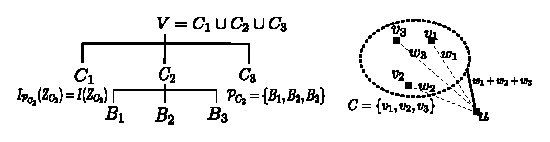
\includegraphics[width=0.9\linewidth]{img/two_approach.eps}

\begin{equation*}
	\P = 
	\begin{cases}
		\{\{1,2,3,4\}\} & \lambda < 0.9 \\
		\{\{1,2\},\{3,4\}\} & 0.9 \leq \lambda < 1 \\
		\{\{1\},\{2\},\{3,4\}\} & 1 \leq \lambda < 2\\
		\{\{1\},\{2\},\{3\},\{4\}\} & \lambda \geq 2
	\end{cases}
\end{equation*}

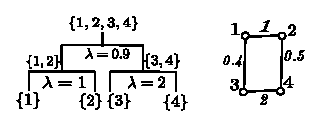
\includegraphics[width=0.77\linewidth]{img/threshold.eps}
}

%%%%%%%%%%%%%%%%%%%%%%%%%%%%%%%%%%%%%%%%%%%%%%%%%%%%%%%%%%%%%%%%%%%%%%%%%%%%%%
\headerbox{Algorithm}{name=results,column=1,span=2,row=0}{
%%%%%%%%%%%%%%%%%%%%%%%%%%%%%%%%%%%%%%%%%%%%%%%%%%%%%%%%%%%%%%%%%%%%%%%%%%%%%%

\begin{multicols}{2}

The clustering result can be achieved by solving the principal sequence of partition for the input graph.
\begin{align}\label{eq:hL}
	h_{\P}(\lambda) &=  f[\P] - \abs{\P} \lambda  \\
	h(\lambda) &= \min_{\P \in \Pi'(V)} h_{\P}(\lambda)
\end{align}
Solving the following problem sequentially for $t=1,\dots,\abs{V}$ (\textsf{pdt}).
\begin{align}
	\tilde{h}_{\lambda}(T) &= f(T) - \lambda - y^{\lambda}(T)\\
	\tilde{h}(\lambda) & = \min_{t \in T \subseteq V} \tilde{h}_{\lambda}(T) \label{eq:pmq}
\end{align}
\begin{theorem}[Principal Sequence]
	\begin{align}\notag
		T^{\lambda} & =\begin{cases}
			T_0 & \lambda < \lambda_1 \\
			T_i & \lambda_i \leq \lambda < \lambda_{i+1}\\
			T_k & \lambda \geq \lambda_{k}
		\end{cases} \\
		T_k & \subsetneq  \dots \subsetneq T_1 \subsetneq T_0 \label{eq:Alambda}				
	\end{align}
\end{theorem}
{
		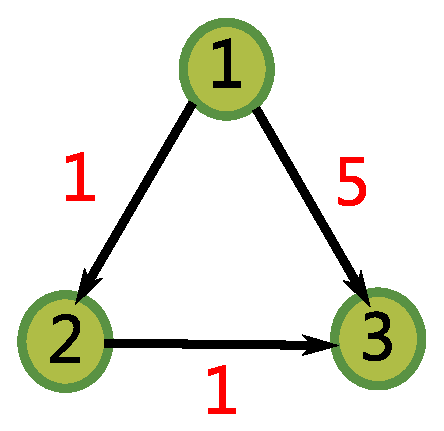
\includegraphics[width=0.27\linewidth]{img/example_directed.eps}~
		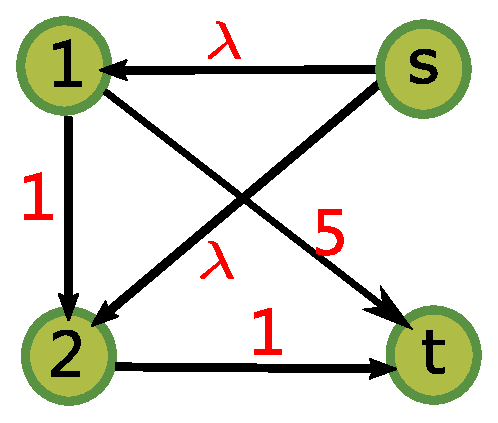
\includegraphics[width=0.3\linewidth]{img/example_st.eps}~
		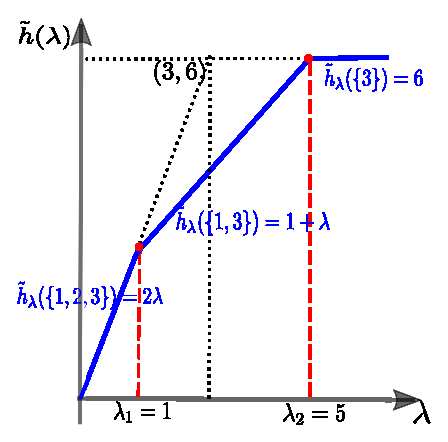
\includegraphics[width=0.27\linewidth]{img/example_pst_single.eps}
}

To compute $\tilde{h}(\lambda)$, we combine Algorithm \ref{alg:pmfT} and \textsf{pmf}.
\begin{algorithm}[H]
	\caption{
		{\footnotesize
		Parametric Computing of $T^{\lambda} = \argmin_{t\in T} g_{\lambda}(T)$
		}
	}\label{alg:pmfT}
	\begin{algorithmic}[1]
		\REQUIRE set $V$, $t \in V$, function $g_{\lambda}$ whose domain is $V$.
		\ENSURE An ordered array \textbf{L} which contains $\lambda_1, \dots \lambda_k$ and a reversely ordered array $T^{\lambda}$ which contains $T_0,\dots, T_k$. (defined in equation \eqref{eq:Alambda})
		\STATE \textbf{L}, $A^{\lambda} \leftarrow$ empty arrays of size $\abs{V}$
		\STATE $Q \leftarrow \argmin_{A\in V} g_{-\epsilon}(A), P \leftarrow \{ t \}$ \label{alg:uini}
		\STATE add $Q$ and $P$ to $T^{\lambda}$
		\STATE \texttt{Split}$(Q,P)$
		\FUNCTION{\texttt{Split}$(Q,P)$}
		\STATE Let $\tilde{\lambda}_2$ be the solution to $g_{\lambda}(Q) =  g_{\lambda}(P)$
		\STATE $h' = g_{\tilde{\lambda}_2}(Q)$
		\STATE $P' =\argmin_{A\in V} g_{\tilde{\lambda}_2}(A)$  \label{alg:Pap}
		\IF{$ g_{\tilde{\lambda}_2}(P') = h'$}
		\STATE add  $\tilde{\lambda}_2$ to $\mathbf{L}$
		\ELSE
		\STATE add $P'$ to $T^{\lambda}$ \label{alg:addP}
		\STATE \texttt{Split}$(Q,P')$
		\STATE \texttt{Split}$(P',P)$
		\ENDIF
		\ENDFUNCTION
	\end{algorithmic}
\end{algorithm}
{

}
\begin{multicols}{2}		
Converting $G$ to $\widetilde{G}$ by adding $s$ and modifying weights.
Starting from a given flow map when computing $P'$.

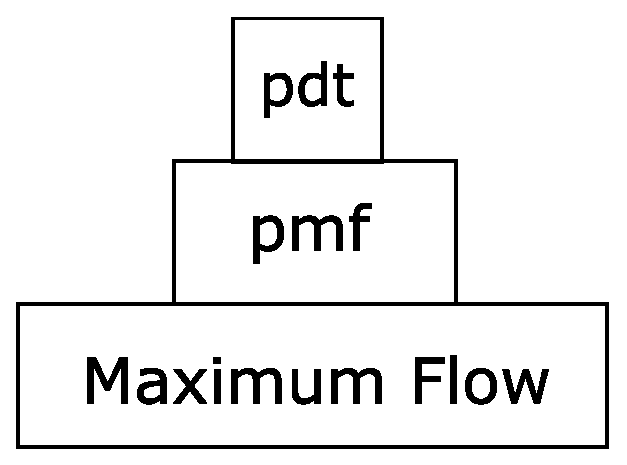
\includegraphics[width=0.65\linewidth]{img/pdt.eps}
\end{multicols}
\end{multicols}

}

\headerbox{How to choose graph weight}{name=example,below=results,column=1,span=2}{
	%%%%%%%%%%%%%%%%%%%%%%%%%%%%%%%%%%%%%%%%%%%%%%%%%%%%%%%%%%%%%%%%%%%%%%%%%%%%%%
	\begin{multicols}{2}
The clustering tree has no stem nodes if and only if
\begin{equation}
	\frac{f[\P]}{\abs{\P}-1} \geq \frac{\sum_{(i,j) \in E} w_{ij}}{\abs{V}-1}				
\end{equation}
holds for any partition $\abs{\P} > 1$.

If $w_{ij} + w_{jk} \geq w_{ki}$ for any different triple $i, j, k \in V$, then the clustering tree has no stem nodes.

Suppose $S_1, S_2 $ are complete graph with size $n$ equal weight $w_{ij}=n$. There are $m$ edges between the two graphs and all inter-connection edges have equal weight 1. Then for $V=S_1\cup S_2$, we have
\begin{equation*}
	I(Z_V) = \begin{cases}
		m & m <\frac{n^2}{2}, S_1,S_2 \textrm{are non-trivial} \\
		\frac{m+n^2(n-1)}{2n-1} & m\geq \frac{n^2}{2}, \textrm{only trivial cluster} 
	\end{cases}
\end{equation*}
	\end{multicols}
}

%%%%%%%%%%%%%%%%%%%%%%%%%%%%%%%%%%%%%%%%%%%%%%%%%%%%%%%%%%%%%%%%%%%%%%%%%%%%%%
  \headerbox{Experimental Results}{name=experiment,column=1, span=2,below=example, above=bottom}{
%%%%%%%%%%%%%%%%%%%%%%%%%%%%%%%%%%%%%%%%%%%%%%%%%%%%%%%%%%%%%%%%%%%%%%%%%%%%%%
\begin{multicols}{2}
We tested our method "graph-based info-clustering" to cluster multi-dimensional vectors. We prepare three groups of data.

\textbf{1)} Four Gaussian blobs 

\textbf{2)} Three concentric circles

\textbf{3)} UCI glass dataset with 214 samples, 6 classes

{ 
	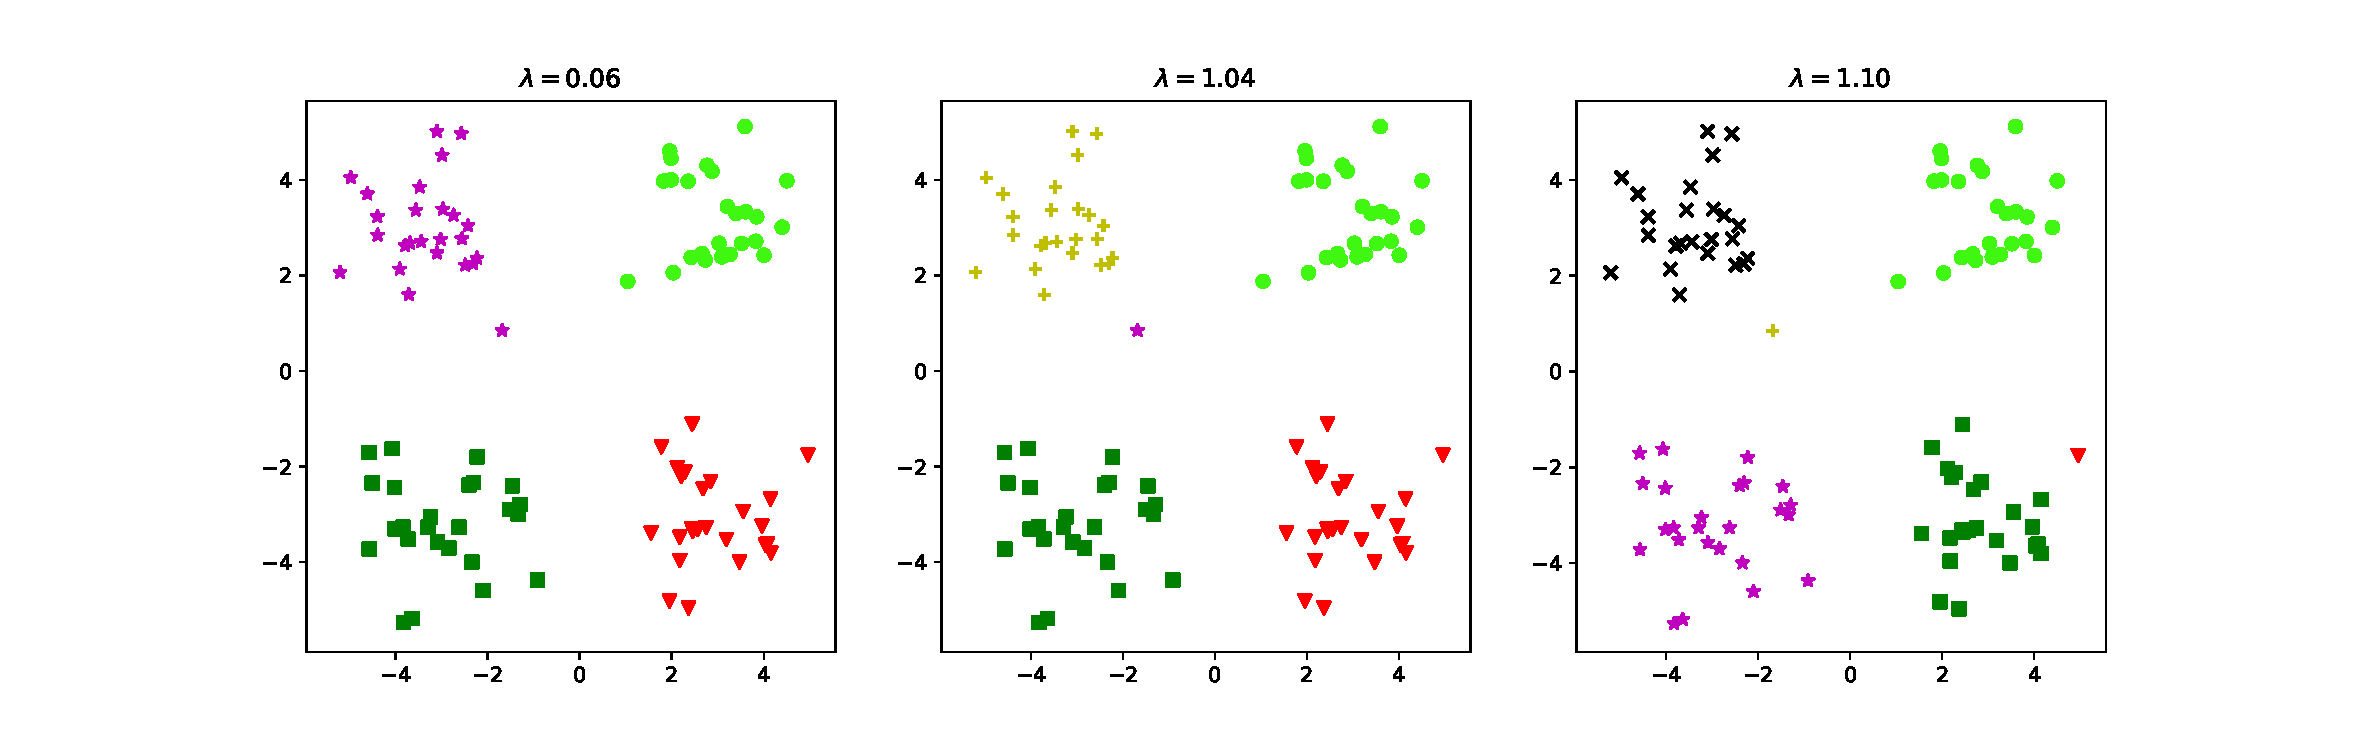
\includegraphics[width=0.96\linewidth]{img/4part}
	}	
	
	{	
	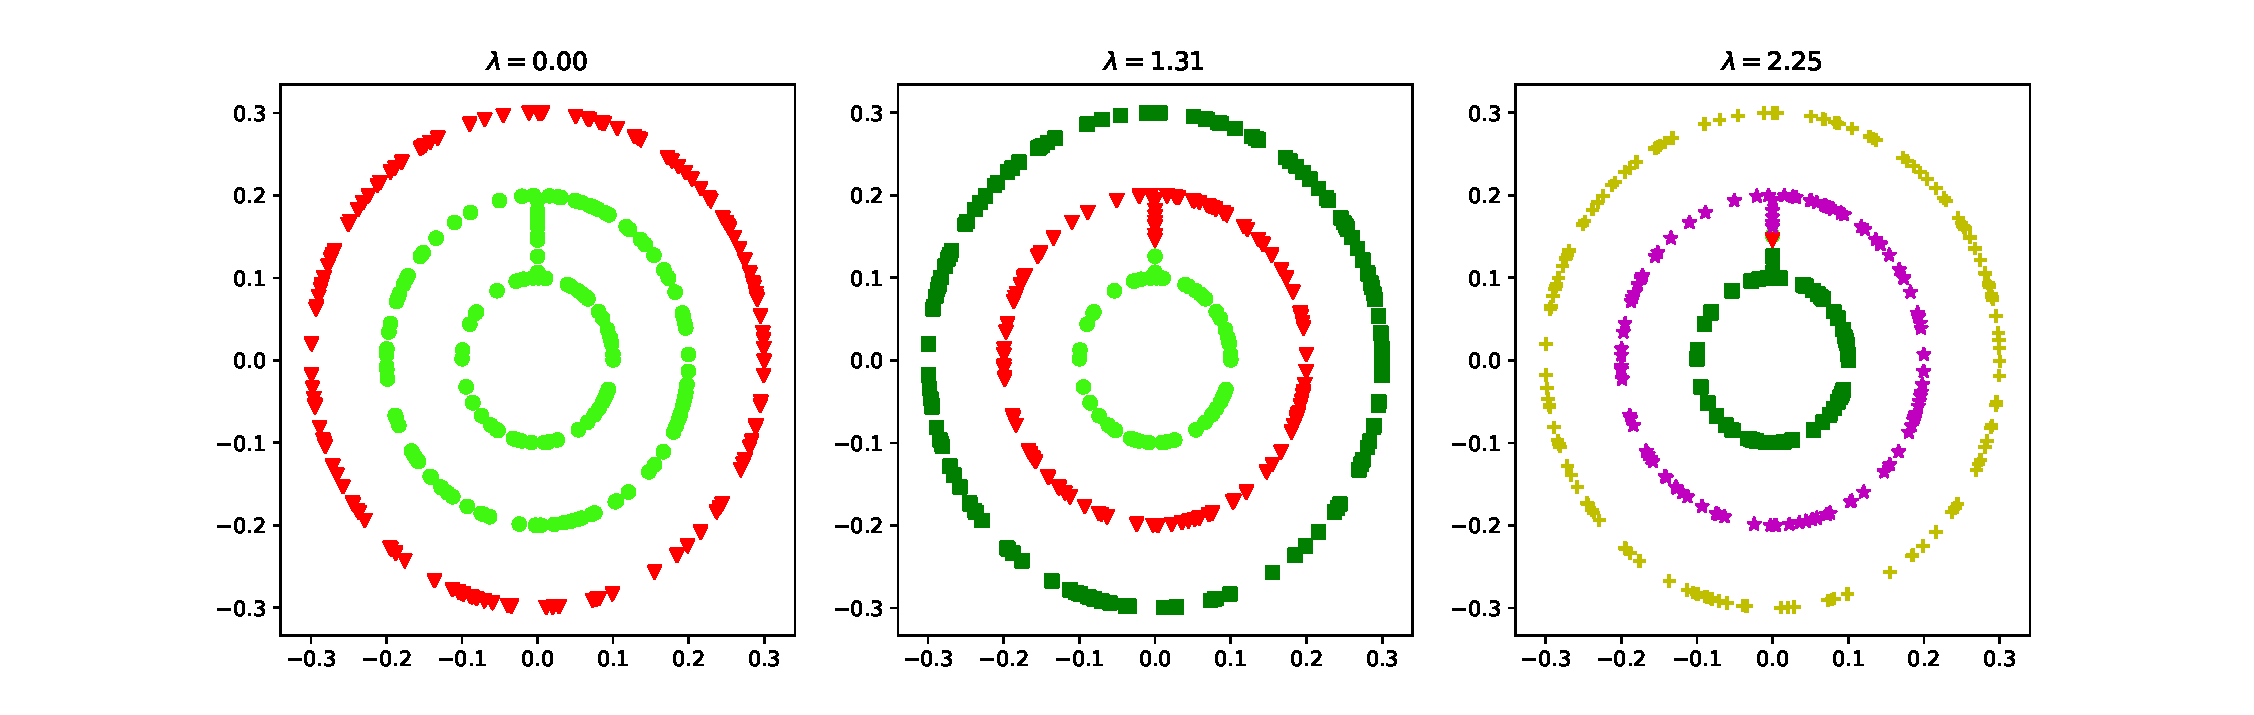
\includegraphics[width=0.96\linewidth]{img/3circle}
}


clustering result of Gaussian and Circle dataset is shown on above figure.
\\

\begin{tabular}{lp{1.1cm}cc}
\hline
 Adjusted rand index   &   Gaussian &   Circle &   Glass \\
\hline
 agglomerative         &       1.00 &     1.00 &    0.21 \\
 affinity propagation  &       1.00 &     0.14 &    0.19 \\
 info-clustering       &       1.00 &     1.00 &    0.30 \\
\hline
\end{tabular}
\\

In all three dataset, graph-based info-clustering reaches the highest score.

We also evaluated our method on community detection problems. 

{
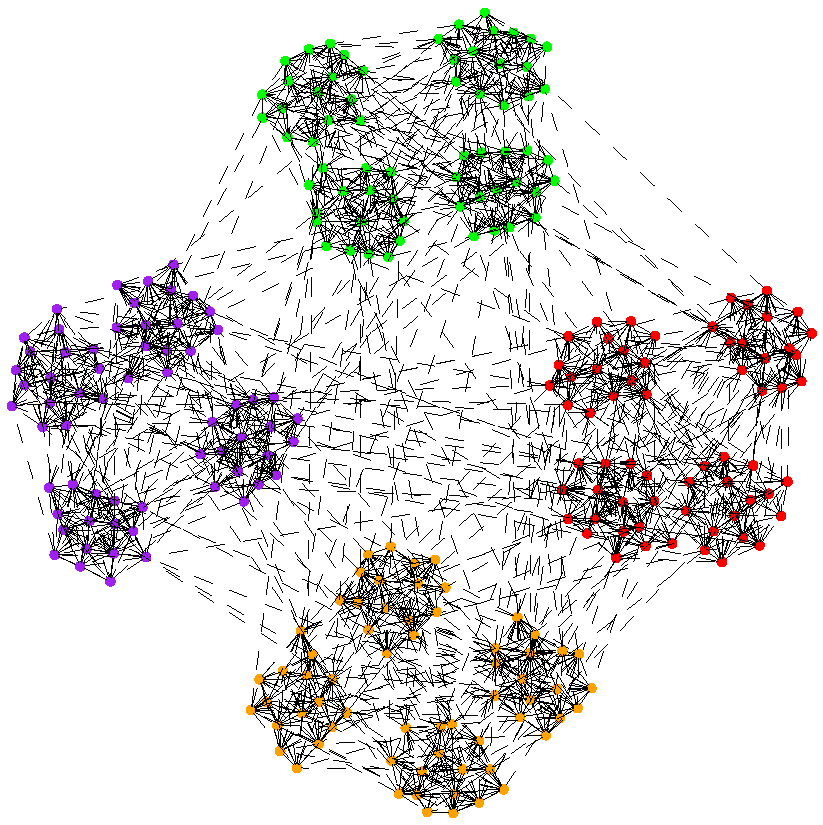
\includegraphics[width=0.4\linewidth]{img/two_level.pdf}
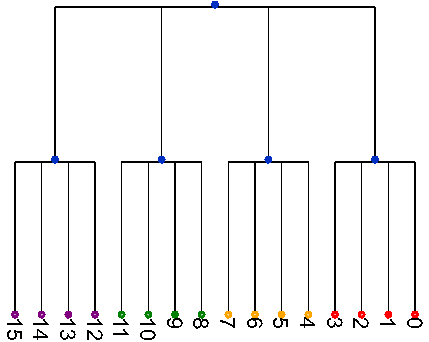
\includegraphics[width=0.46\linewidth]{img/tree_info-clustering.pdf} 
}

The community has a two-level structure with configuration paramter $\{z_{\mathrm{in}_1}, z_{\mathrm{in}_2}, z_{\mathrm{out}} \}$.
In some parameter combination, the hierarchical tree obtained by graph-based info-clustering is the same as that of the ground truth.\\

{
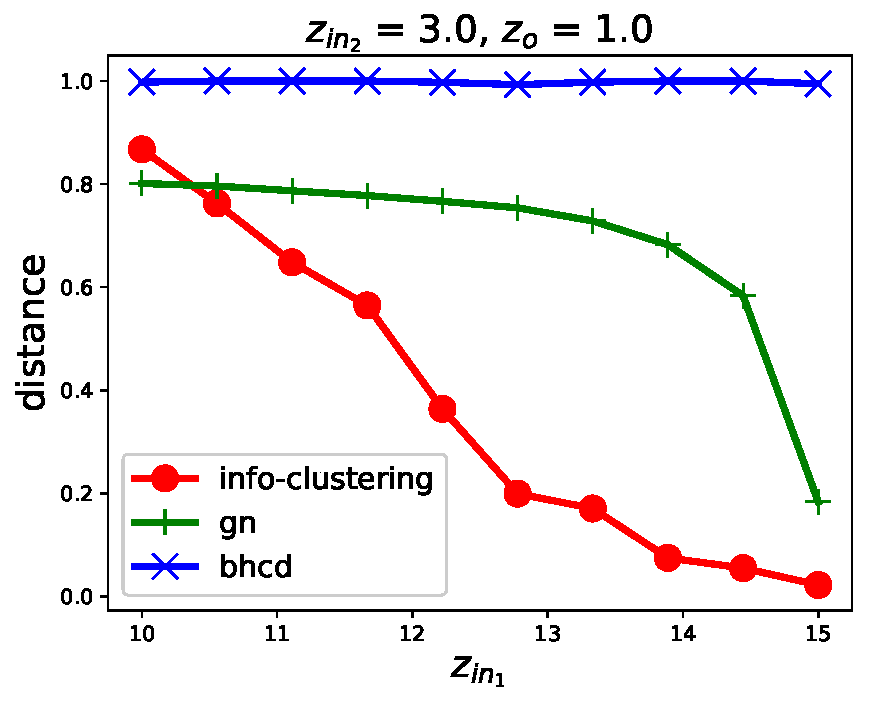
\includegraphics[width=0.46\linewidth]{img/z_in_1.pdf}
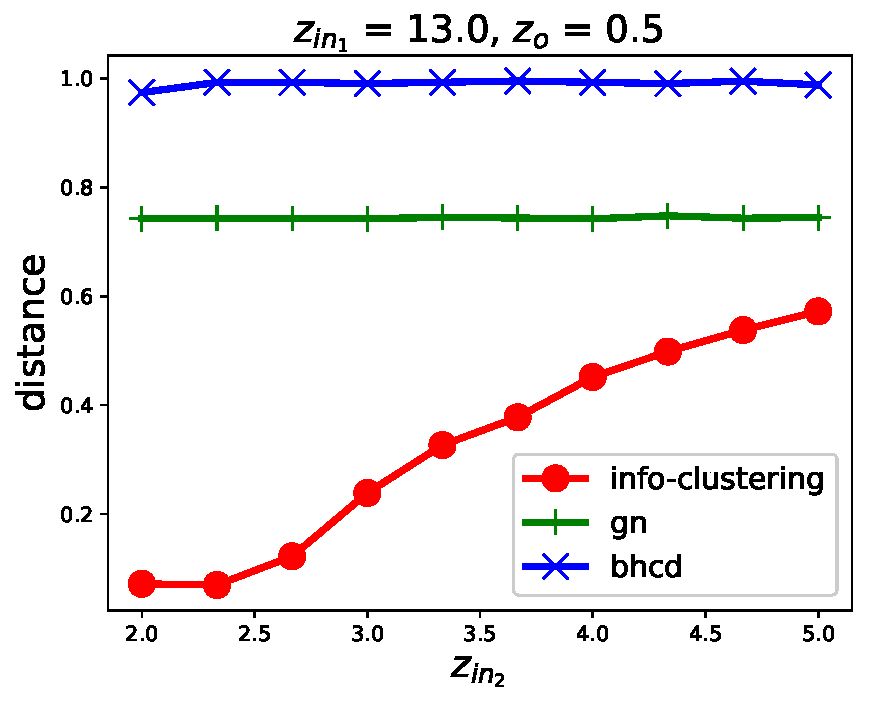
\includegraphics[width=0.46\linewidth]{img/z_in_2.pdf}
}

{
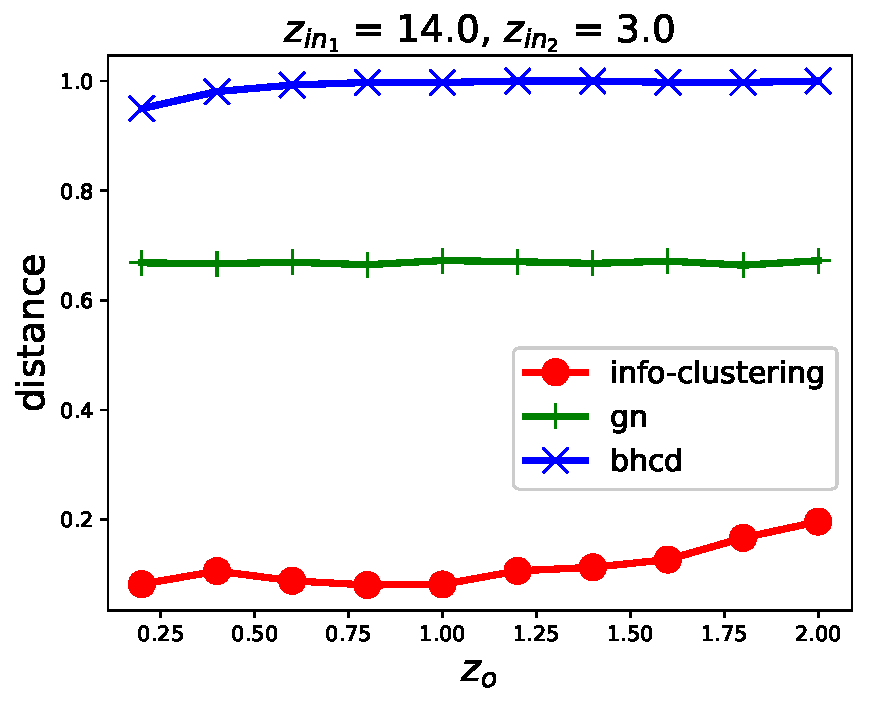
\includegraphics[width=0.46\linewidth]{img/z_o.pdf}~

\includegraphics[width=0.4\linewidth]{github_qrcode.png}
}

As shown, graph-based info-clustering produces more similar tree structures.
\end{multicols}

}


\end{poster}

\end{document}

